\section{Results}\label{sec:results}
To systematically evaluate the different configurations of each clustering algorithm, the following procedure is followed to extract results for each of the 3 data sets, in order to later perform an analysis those results:

\begin{enumerate}
    \item \textbf{Data Preparation}: The dataset is loaded and the data samples are separated from their labels into separate 2 sets. This way, we perform the clustering analysis in a completely non-supervised way, and we then utilize the labels to extract supervised metrics of the cultering results.

    \item \textbf{Parameter Configuration}: A comprehensive set of values for the algorithm's hyperparameters is defined. These combinations reflect various ways to tune the clustering algorithm.

    \item \textbf{Model Evaluation}: For each parameter combination, the clustering algorithm is applied on the unlabeled data and then evaluated with different metrics. This step yields the following metrics: Adjusted Rand Score (ARI), Normalized Mutual Information (NMI), Davies-Bouldin Index(DBI), Silhouette score, Calinski-Harabasz Score (CHS), and execution time. Together, these metrics (the first 2 supervised, and the rest non-supervised) measure the effectiveness and efficiency of the clustering.

    \item \textbf{Results Compilation}: The performance metrics for each parameter combination are recorded in a structured format. These results are saved as a dataset that summarizes the outcomes of all evaluations, forming a basis for analysis. We save as well the cluster labels of all samples for each clustering algorithm that we run, so we can recover the same clusters in the posterior analysis.

    \item \textbf{Results Analysis}: After results are compiled across all configurations, quantitative and qualitative analysis is performed to identify common trends among the different algorithm configurations for each of the datasets. Additionally, we extract the top performing configuration according to each of the 5 evaluation metrics, in order to study common patterns and visualize the resulting clusters. This analysis helps determine the most reliable and effective parameter settings for accurate and efficient clustering for each dataset.
\end{enumerate}
Due to the vast ammount of information that can be extracted from the results, we will only explicitly showcase the most clarifying plots and results that we have extracted. However, all of the information is available in the \texttt{plots\_and\_tables} folder for each of the datasets, in the \texttt{code} attached to this report.

\textit{Note:} Since all of the tested datasets have high dimensionality, we use Principal Component Analysis (PCA) to extract the 2 principal components in order to generate the clustering scatter plots of the datasets for visualization purposes.

\subsection{K-Means}
We have tested on each dataset 57 different configurations of the K-Means algorithm, by using the 3 different distance metrics with 19 different values of the k (from 2 to 20). For each of these configurations, we have run the K-Means 10 times, in order to account for the randomness of the centroid initialization. This results in a total of 570 runs of the K-Means algorithm for each dataset. From the evaluation metrics extracted for each of these runs, we study the effect of each of the 2 hyperparameters and achieve conclusions about them through statistical analysis.

\subsubsection{Preliminary Study}
Before starting with the more rigorous statistical analysis, let us first observe some preliminary patterns about the measured metrics and the effect of each hyperparameter on the clustering performance.

In Figure \ref{fig:metrics_corr} we summarize the relationship between the different metrics that were measured. It is a matrix plot where the lower triangle is a heatmap of the Pearson correlations between each pair of metrics, the diagonal elements are the histogram distributions of values of each metric, and the upper triangular has for each pair of metrics the plot of their values for all runs. It is interesting to observe that, while we would expect all of the metrics to agree on the identified trends, there are some cases where the opposite behaviour is displayed. An example of this is the negative correlation between E (total variance) and DBI (Davies-Bouldin Index): since the DBI measures cluster compactness, we would expect it to directly correlate to E; however, we observe that there is a negative correlation between them. This specific figure was extracted from the results on the Mushroom dataset, but the conclusions are the same for the others (the plots can be found in the \texttt{code} floder).

\begin{figure}[h]
    \centering
    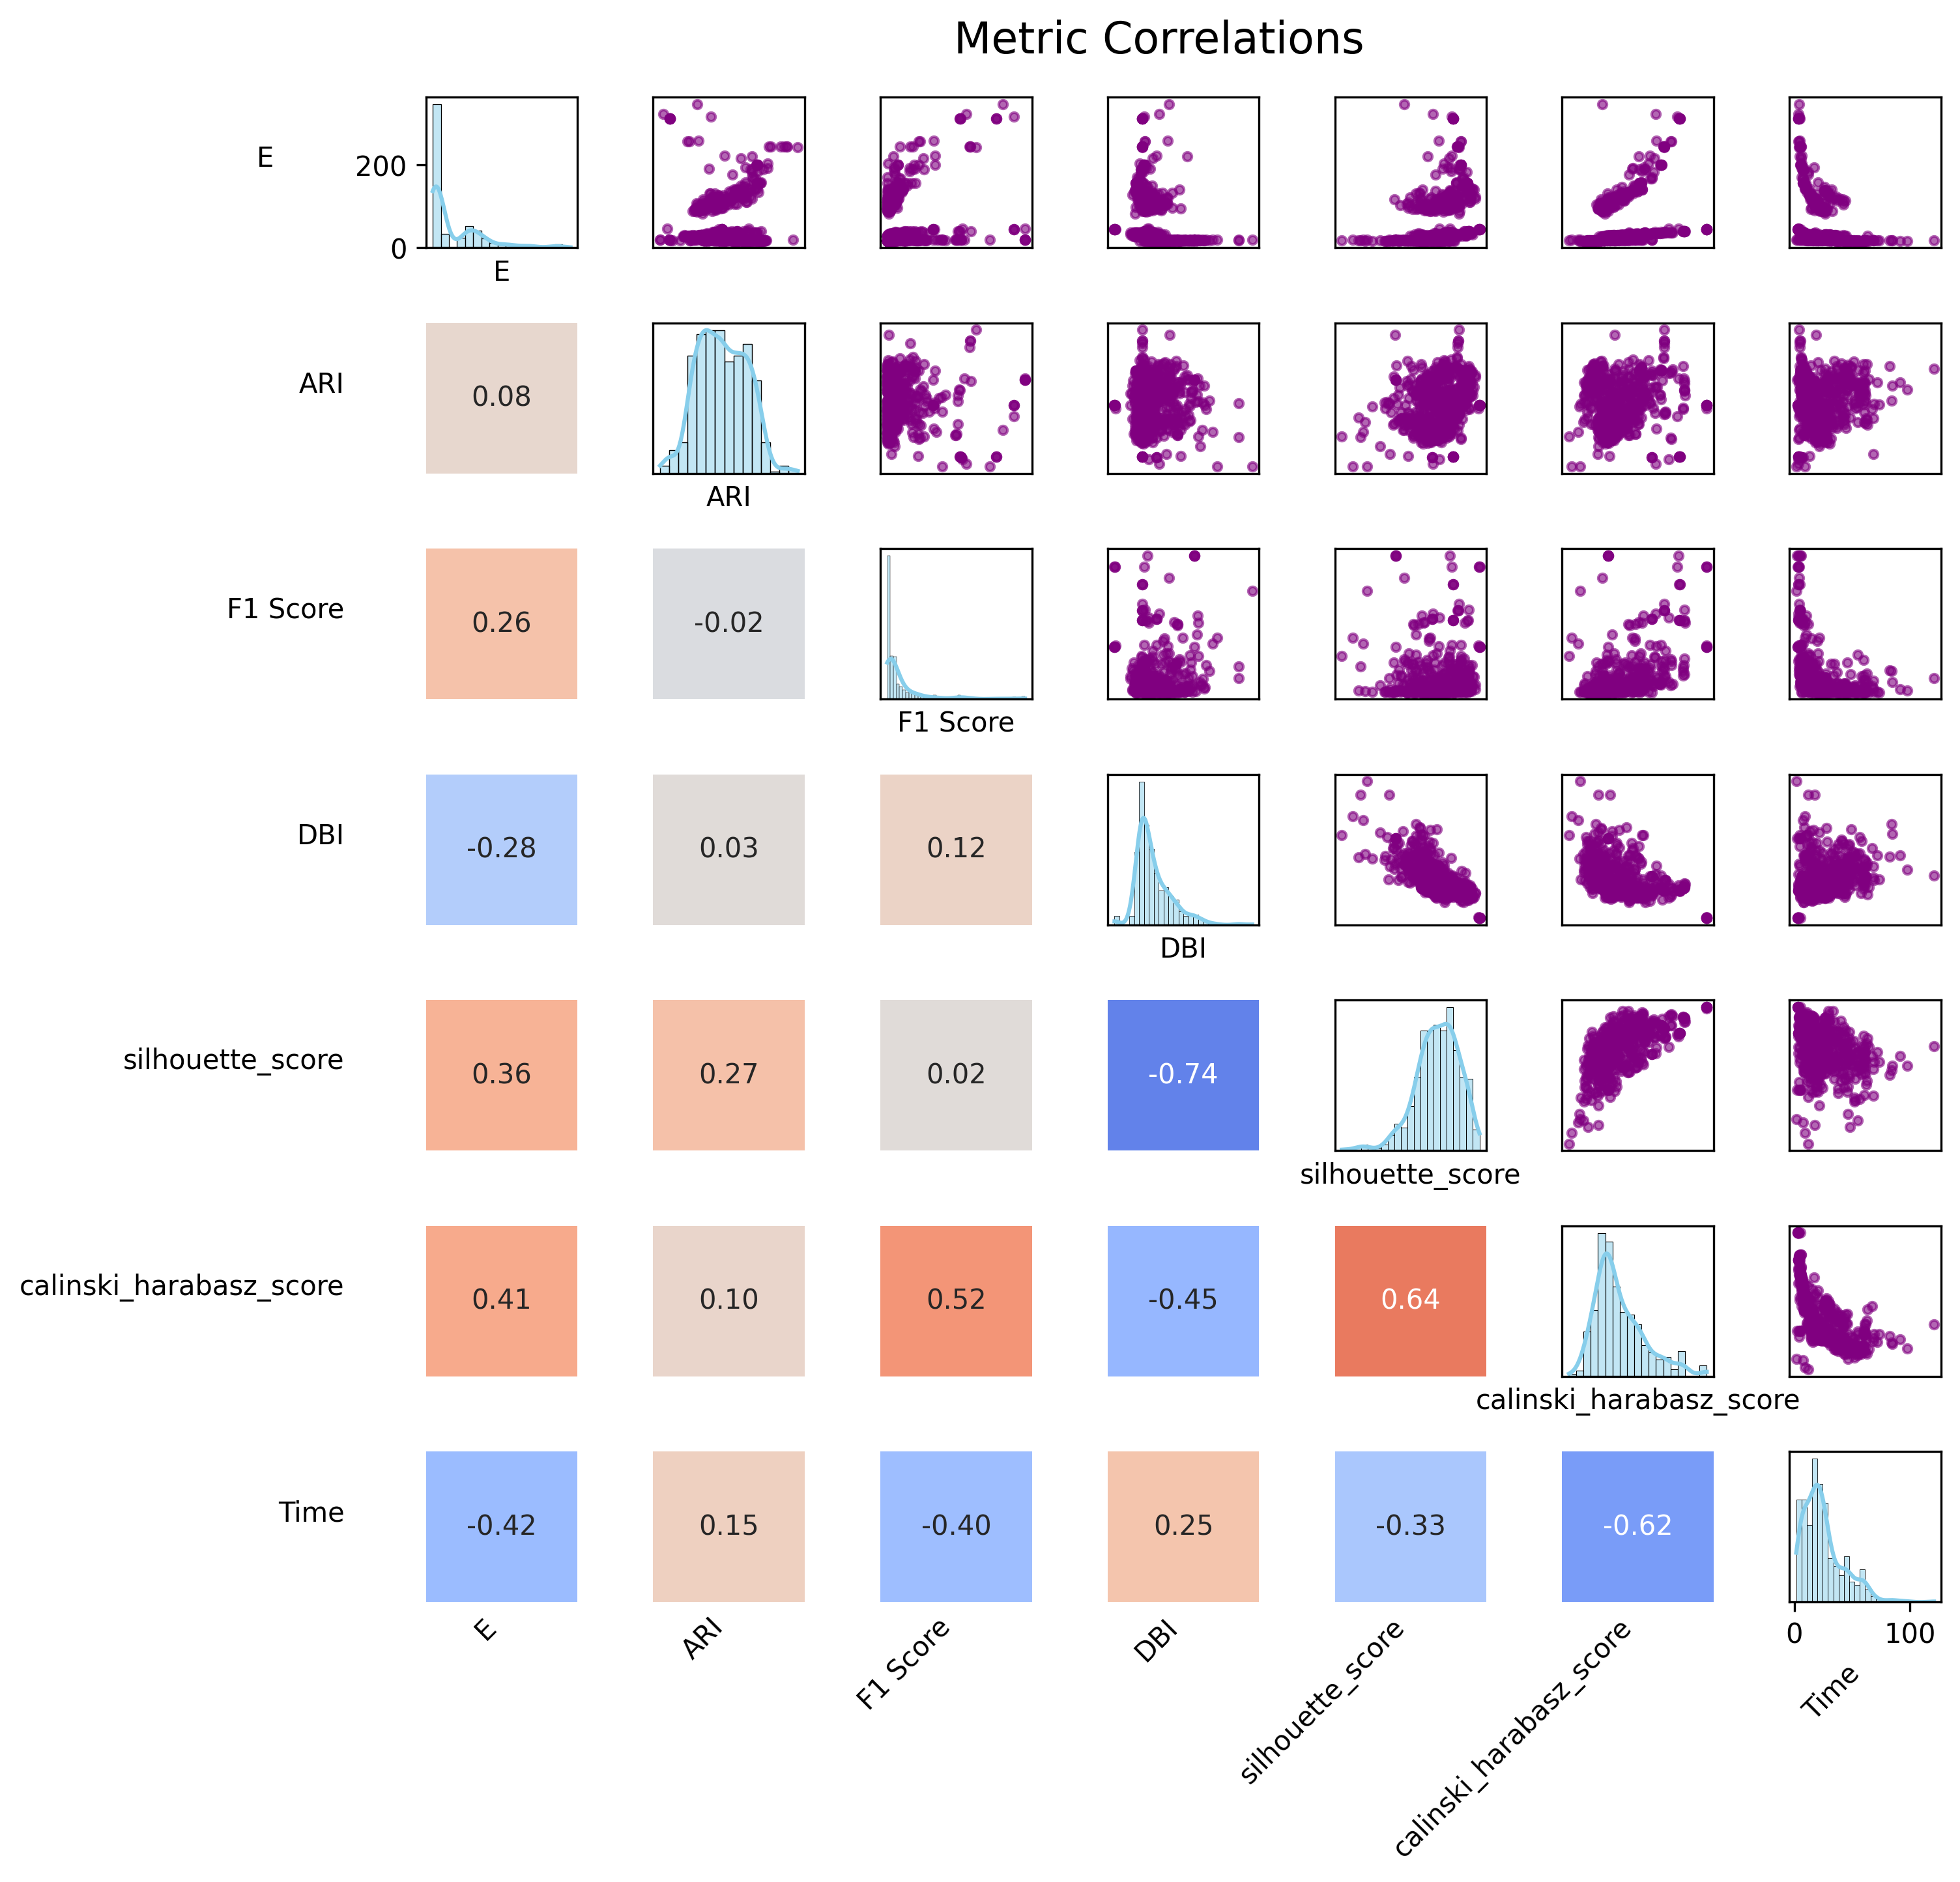
\includegraphics[width=0.7\textwidth]{figures/metrics_correlations_matrix.png}
    \caption{Metrics correlations summary}
    \label{fig:metrics_corr}
\end{figure}

Parallelly, a different set of interesting relationship are displayed in Figure \ref{fig:pairplot}, where we can see heatmaps of the F1 Score and the Time across the different pairwise hyperparameter configurations. We can observe a general trend regarding execution time: it seems to have considerably larger values for the Clark distance metric compared to those of the other 2, which reflects the higher computational cost that this distance metric has. Additionally, we see a noteworthy divergence in the F1 Score trends with respect to the values of k: in the Mushroom dataset (which has 2 classes), lower values of k seem to achieve a better F1 Score; meanwhile, in the Pen-based dataset (which has 10 classes), intermediate values of k (between 7 and 11) seem to achieve the best scores. This was to be expected, yet it still is compelling to see it reflected so clearly in the results. 

\begin{figure}[H]
    \centering
    \begin{subfigure}{0.49\textwidth}
        \centering
        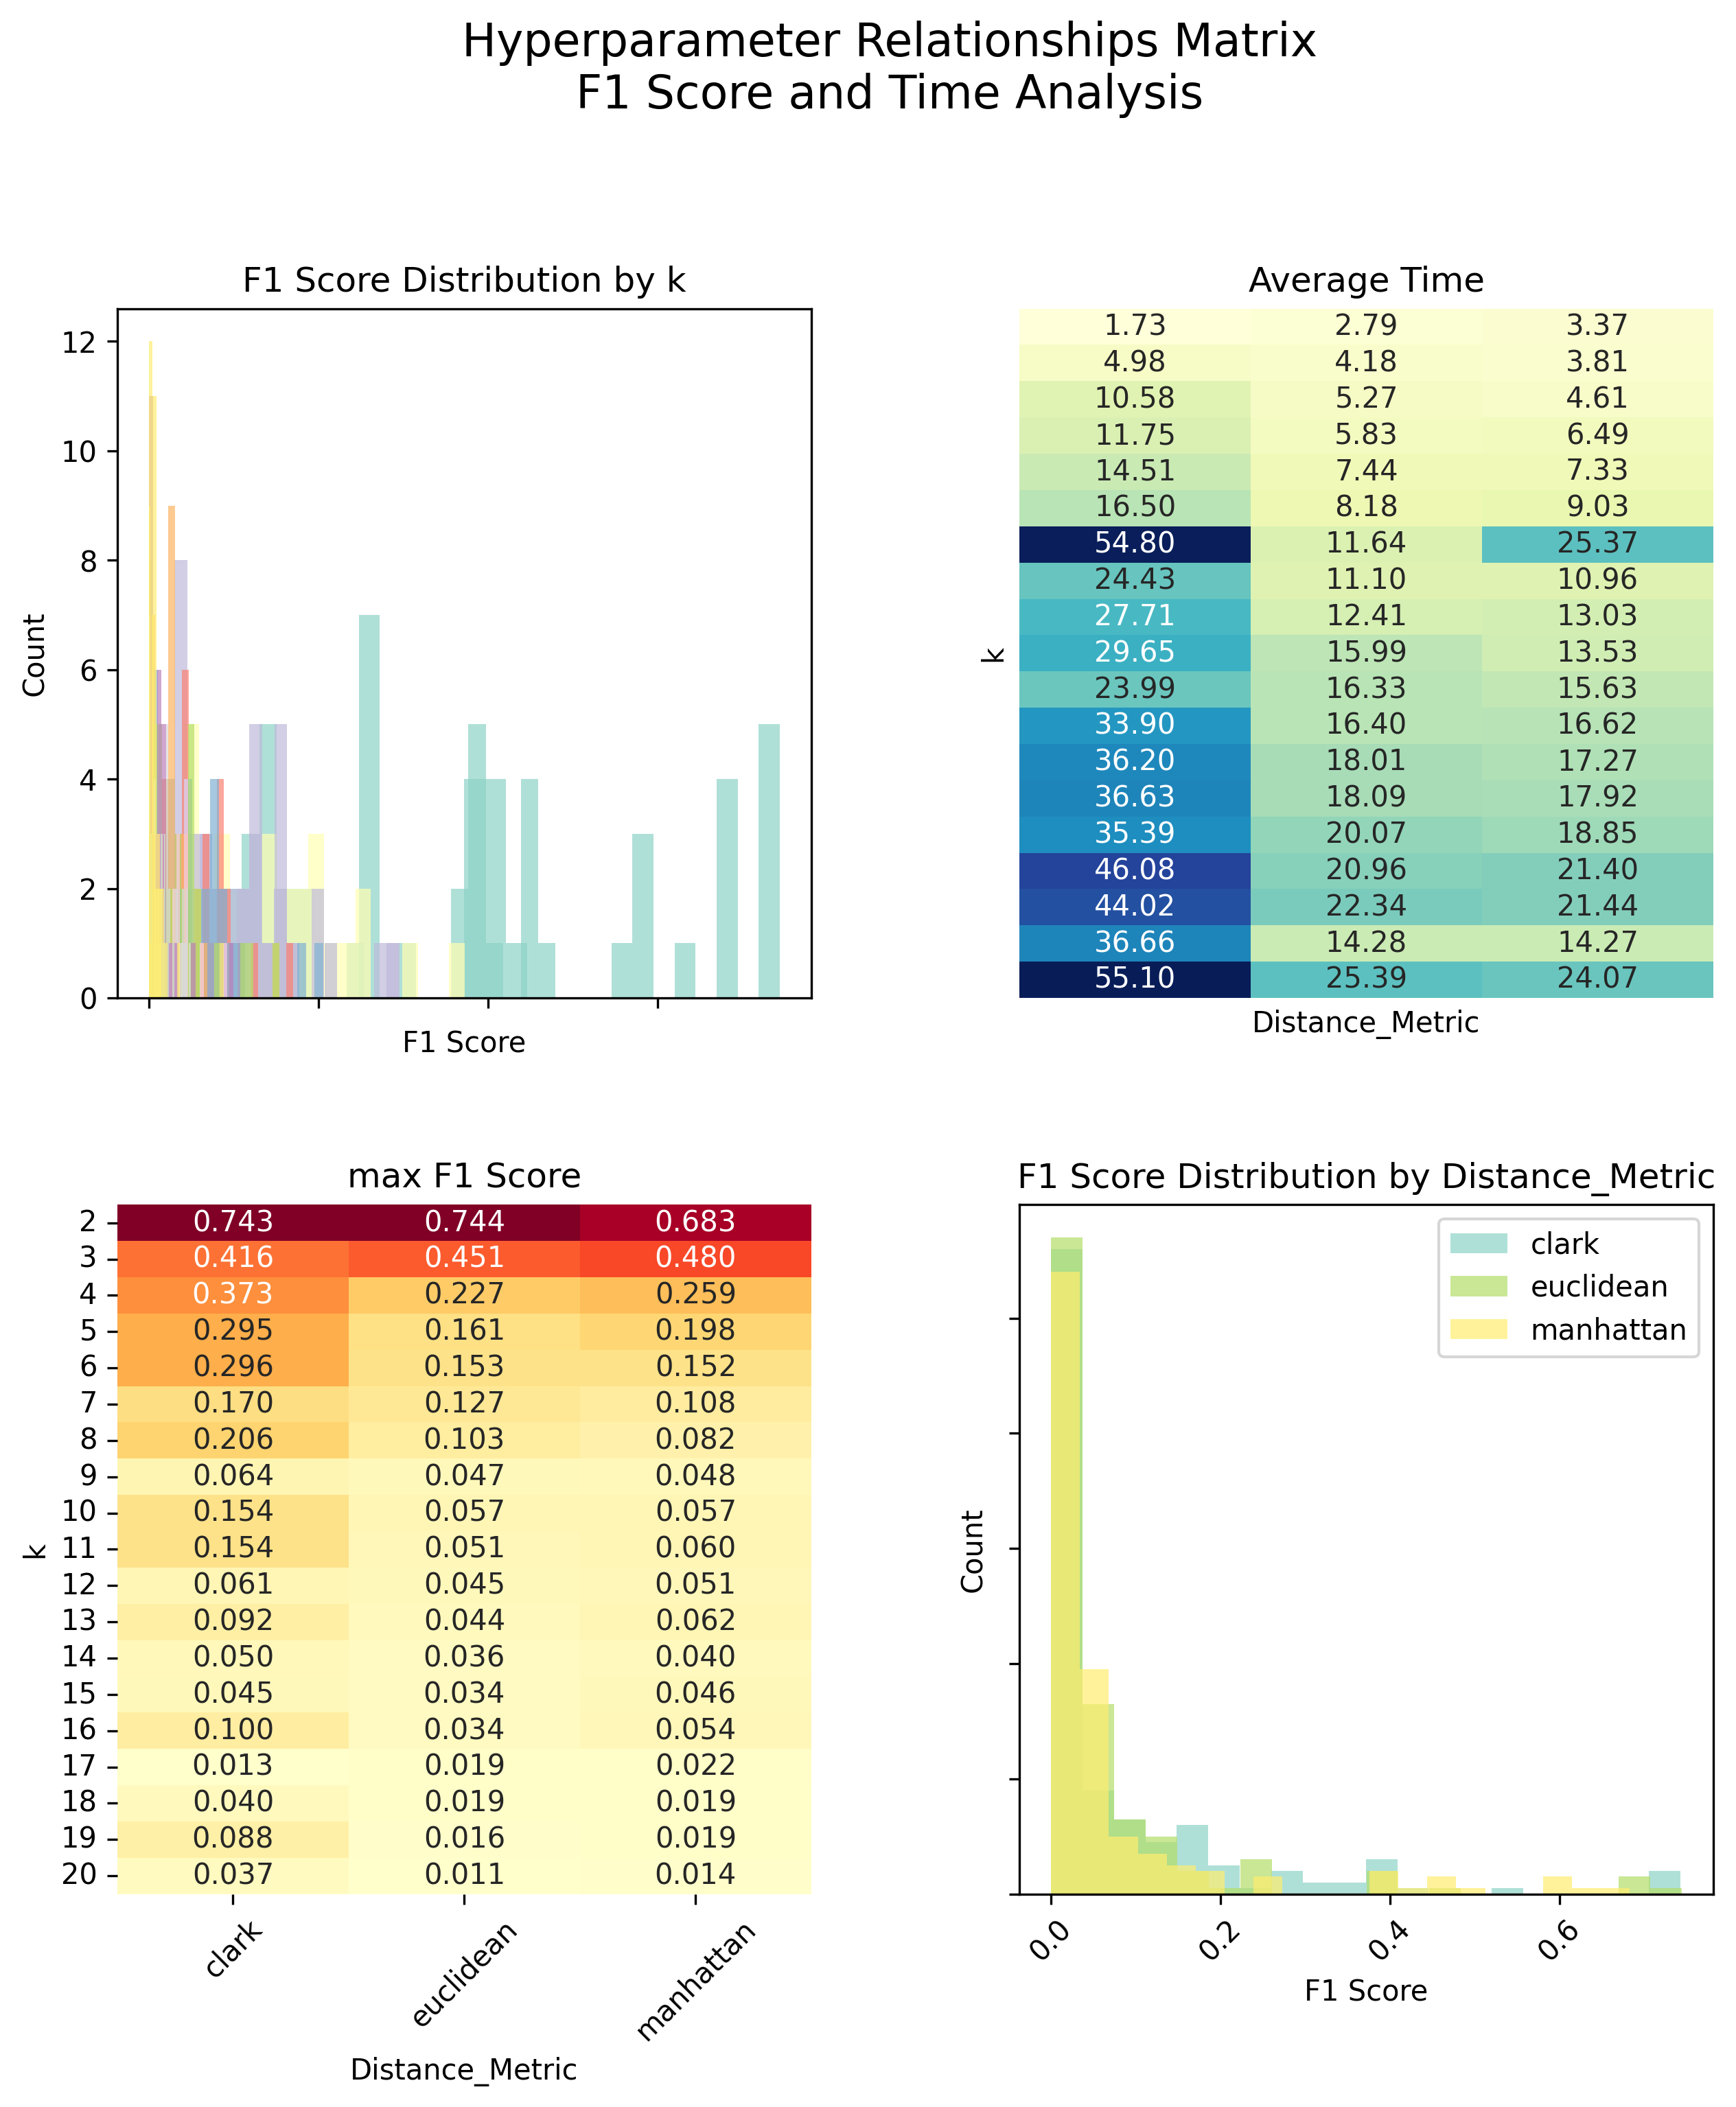
\includegraphics[width=\linewidth]{figures/mushroom_hyperparameter_pairplot_matrix.png}
        \caption{Mushroom pairplot matrix}
    \end{subfigure}
    \hfill
    \begin{subfigure}{0.49\textwidth}
        \centering
        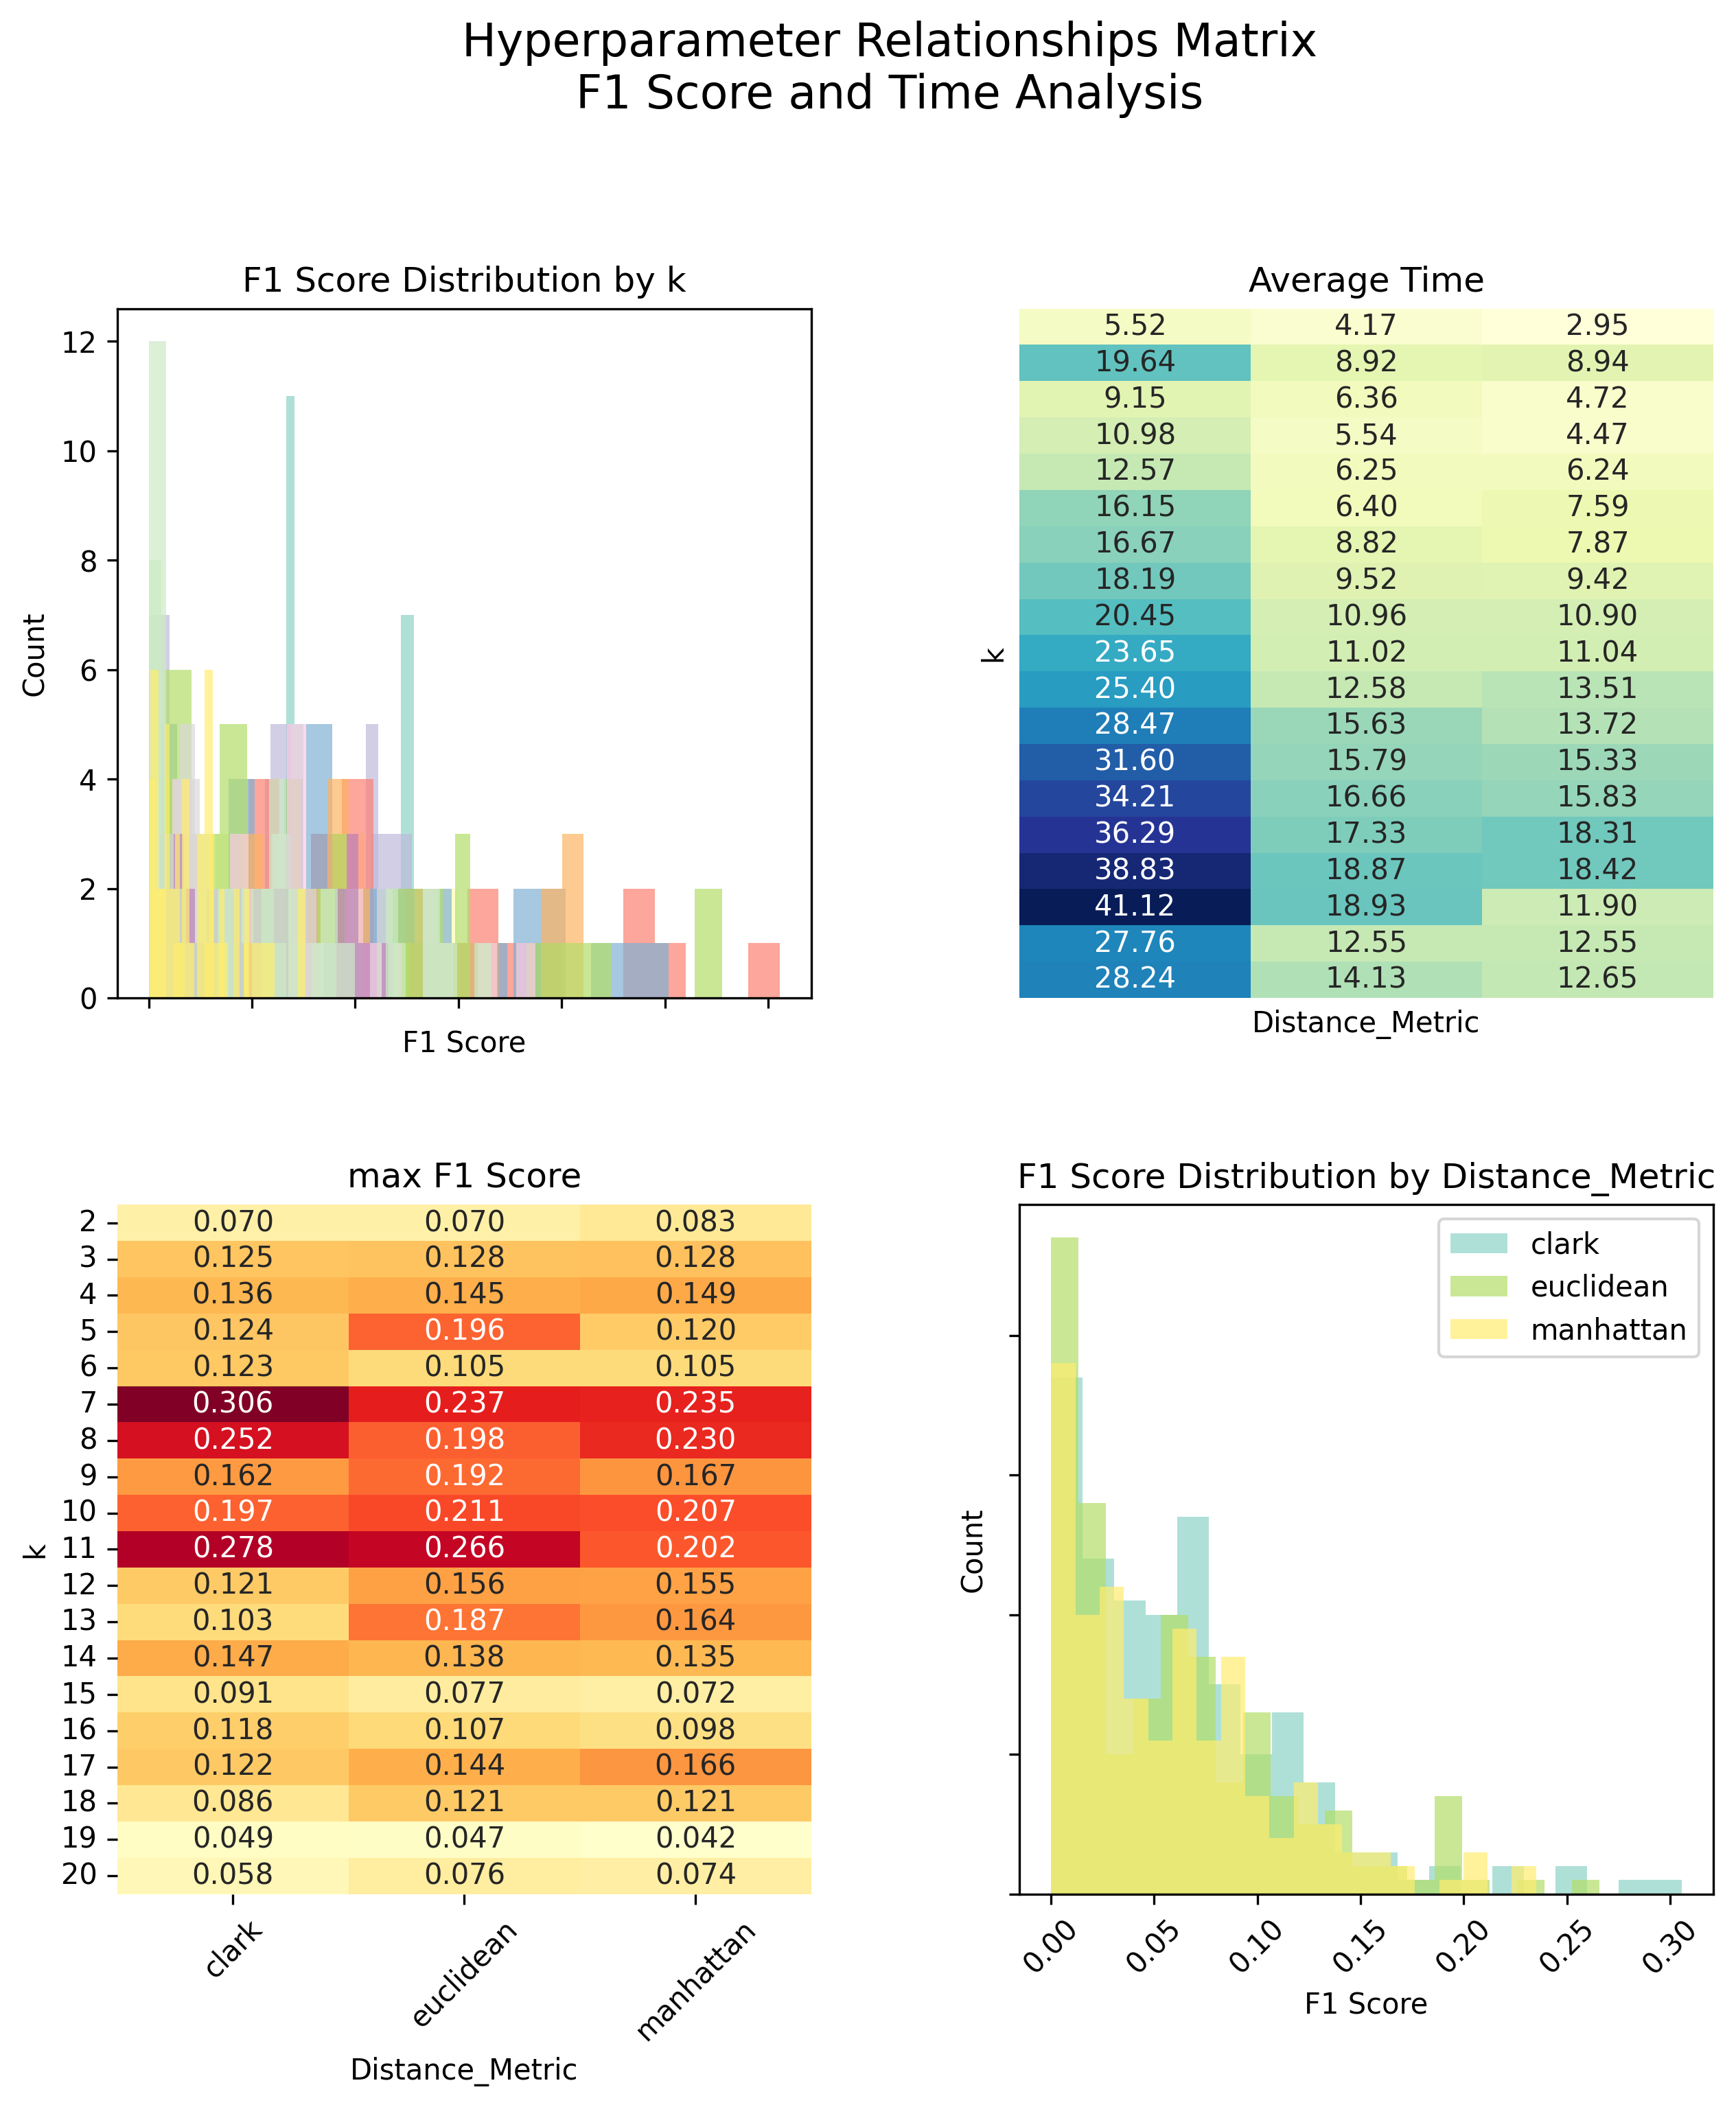
\includegraphics[width=\linewidth]{figures/penbased_hyperparameter_pairplot_matrix.png}
        \caption{Pen-based pairplot matrix}
    \end{subfigure}
    \caption{Hyperparameter pairplot matrices based on F1 Score and Time}
    \label{fig:pairplot}
\end{figure}

\subsubsection{Statistical Analysis}
For the statistical analysis, we have first performed Friedman tests to determine if there are significant differences in each of the metrics for the different possible values of each hyperparameter. 
